\documentclass[a4paper,fleqn]{cas-dc}

% If the frontmatter runs over more than one page
% use the longmktitle option.

%\documentclass[a4paper,fleqn,longmktitle]{cas-dc}

\usepackage[numbers]{natbib}
%\usepackage[authoryear]{natbib}
%\usepackage[authoryear,longnamesfirst]{natbib}

%%%Author macros
\def\tsc#1{\csdef{#1}{\textsc{\lowercase{#1}}\xspace}}
\tsc{WGM}
\tsc{QE}
%%%

% Uncomment and use as if needed
%\newtheorem{theorem}{Theorem}
%\newtheorem{lemma}[theorem]{Lemma}
%\newdefinition{rmk}{Remark}
%\newproof{pf}{Proof}
%\newproof{pot}{Proof of Theorem \ref{thm}}

\begin{document}
\let\WriteBookmarks\relax
\def\floatpagepagefraction{1}
\def\textpagefraction{.001}

% Short title
\shorttitle{Meta--heuristic parameter estimation of solar cells with S--shaped IV characteristics}

% Short author
\shortauthors{O. Olikh}

% Main title of the paper
\title [mode = title]{Estimation of parameters for solar cells with S--shaped current--voltage characteristics using meta--heuristic algorithms}

% First author
%
% Options: Use if required
% eg: \author[1,3]{Author Name}[type=editor,
%       style=chinese,
%       auid=000,
%       bioid=1,
%       prefix=Sir,
%       orcid=0000-0000-0000-0000,
%       facebook=<facebook id>,
%       twitter=<twitter id>,
%       linkedin=<linkedin id>,
%       gplus=<gplus id>]
\author{Oleg~Olikh}
%\cormark[1]
\ead{olegolikh@knu.ua}
%\address[1]{Taras Shevchenko National University of Kyiv, 64/13, Volodymyrska Street, City of Kyiv, Ukraine, 01601}


% Address/affiliation
\affiliation{organization={Taras Shevchenko National University of Kyiv},
            addressline={64/13, Volodymyrska Street},
            city={Kyiv},
%          citysep={}, % Uncomment if no comma needed between city and postcode
            postcode={01601},
 %           state={},
            country={Ukraine}}

% For a title note without a number/mark
%\nonumnote{}

% Here goes the abstract
\begin{abstract}
Defect-assisted recombination processes frequently
limit the photovoltaic device performance.
The low-cost and express methods of impurity contamination control
are in demand at solar cell manufacturing.
In this paper, we applied deep learning-based
approach to extract the iron concentration in silicon solar cell from an
ideality factor values.
\end{abstract}

% Use if graphical abstract is present
%\begin{graphicalabstract}
%\includegraphics{}
%\end{graphicalabstract}

% Research highlights
\begin{highlights}
\item Proposed deep learning-based method to predict iron contamination in Si-SC by using IV curve.
\item The simulated IV characteristics are used to create training and test datasets.
\item The DNN's configurations are proposed.
\item The mean squared relative error of prediction is up to 0.005.
\end{highlights}

% Keywords
% Each keyword is seperated by \sep
\begin{keywords}
Ideality factor \sep Silicon \sep $n^+$--$p$--$p^+$ structure \sep
SCAPS \sep Iron contamination \sep Machine learning
\end{keywords}

\maketitle

% Main text
\section{Introduction}\label{Int}



%According to No Free Lunch (NFL), it is logically proved that
%no metaheuristic can respond to all correct optimization problems. In other words, the especial metaheuristic method can
%demonstrate promising results to solve some problems. But this
%algorithm may show the weaker performance and efficiency for
%some other problems. Hence the researchers try to create the
%better optimization techniques each year


%\section{Models and Methods}\label{MM}
\section{Problem definition}\label{MM}
\subsection{Solar cell model}\label{SCModel}
Fig.~\ref{fig_chem}
vividly reveals the structure of the used model \cite{Castro2010}.
It can be seen from the figure that model contains a current source accompanied by a diode D1, a shunt
resistor $R_\mathrm{p1}$ to show the leakage current, and a series resistor $R_\mathrm{s}$ to consider the
losses associated with the load current.
Besides, the second diode D2 with a second parallel resistance $R_\mathrm{p2}$ is placed opposite to the first one and is essential to
simulate the non-ideal effects of the active layer/cathode interface.
In this model, D1 is responsible for the exponential behavior of the I--V curve,
the main contribution of D2 is to simulate the S--shape.
The analytical solution $V(I)$ of the opposed two--diode equivalent circuit model was
 obtained \cite{CastroSolution} using Lambert $W$-function \cite{LambertNew}:


\begin{figure}[]
	\centering
		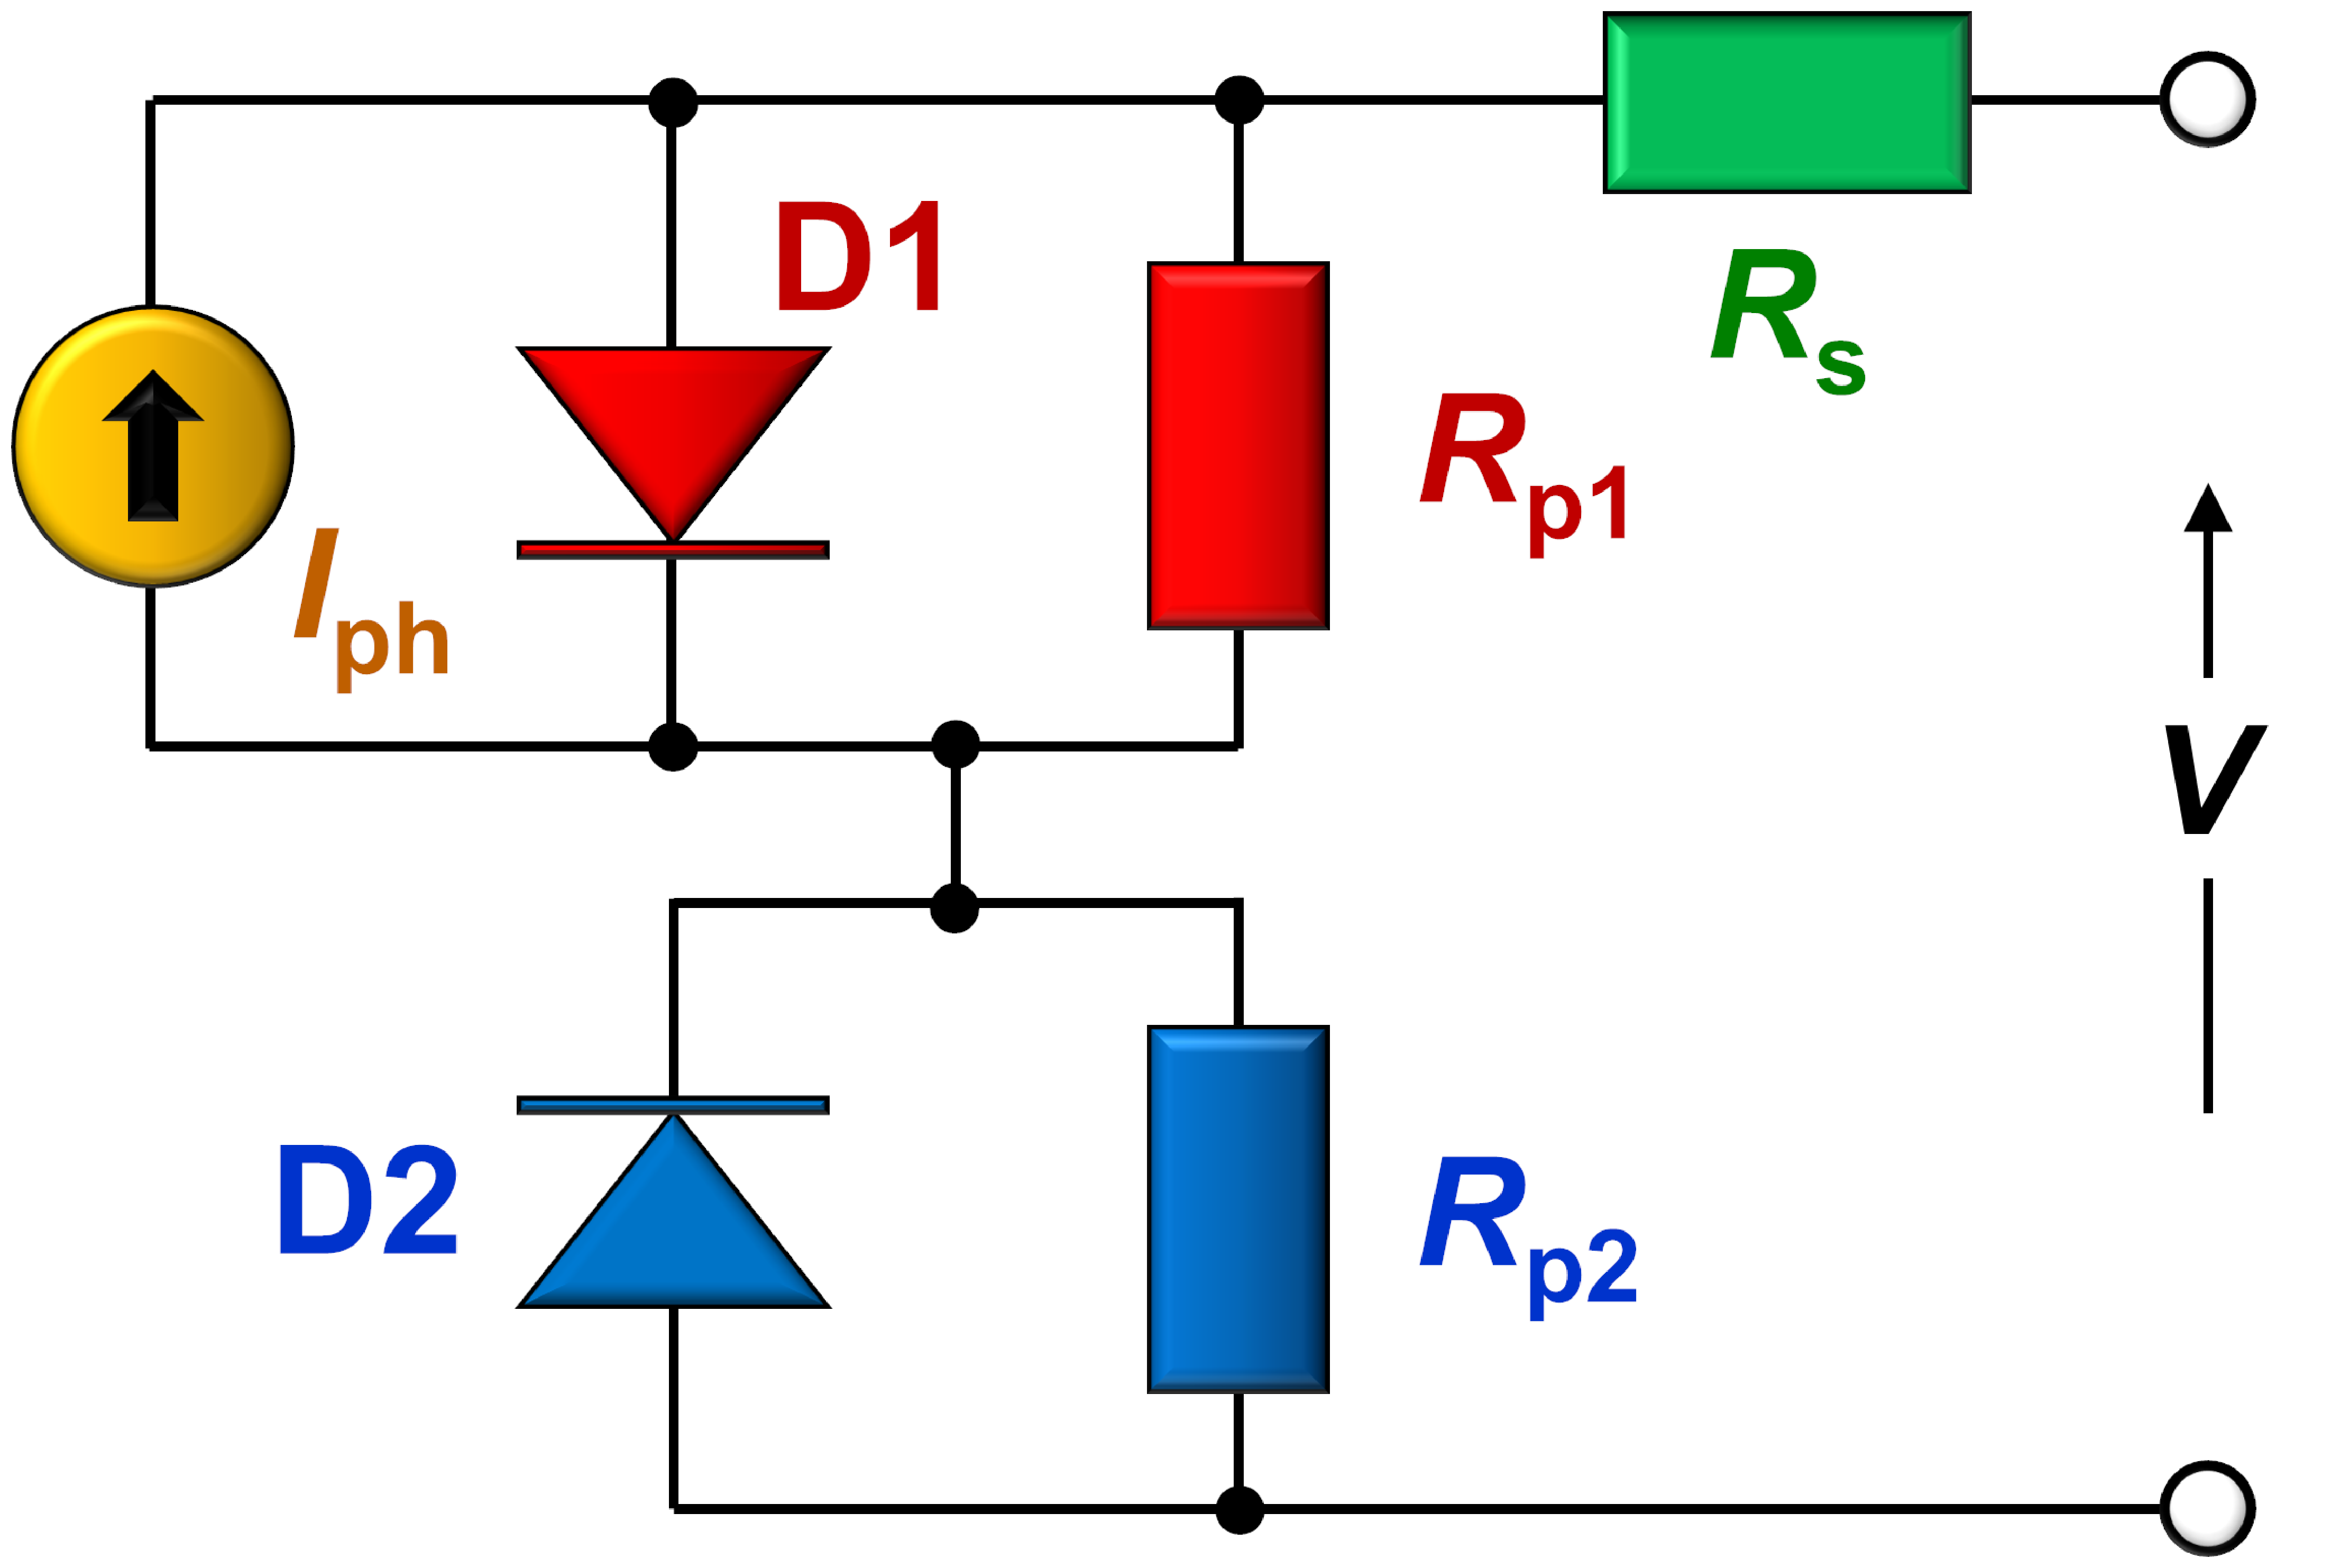
\includegraphics[width=0.9\columnwidth]{Chem}
	  \caption{The opposed two--diode equivalent--circuit model of a solar cell.}\label{fig_chem}
\end{figure}


\begin{eqnarray}
% \nonumber to remove numbering (before each equation)
\label{eqIV_W}
V&=& (I+I_\mathrm{ph}+I_{01})R_\mathrm{p1} \nonumber \\
  &&-\frac{n_1kT}{q}W\left\{\frac{qI_{01}R_\mathrm{p1}}{n_1kT}\exp\left[\frac{qR_\mathrm{p1}(I+I_\mathrm{ph}+I_{01})}{n_1kT}\right]\right\} \nonumber \\
  &&+\frac{n_2kT}{q}W\left\{\frac{qI_{02}R_\mathrm{p2}}{n_2kT}\exp\left[-\frac{qR_\mathrm{p2}(I-I_{02})}{n_2kT}\right]\right\} \nonumber \\
  &&+(I-I_{02})R_\mathrm{p2}+IR_\mathrm{s}\,,
\end{eqnarray}
where
$I_{01}$ and $I_{02}$ are the saturation currents and
$n_1$ and $n_2$ are
the ideality factors for D1 and D2 respectively,
and $I_\mathrm{ph}$ is the ideal photocurrent.
Thus, the model employs eight lumped parameters
($I_{01}$, $n_1$, $R_\mathrm{p1}$, $I_{02}$, $n_2$, $R_\mathrm{p2}$,
$R_\mathrm{s}$, and $I_\mathrm{ph}$)
that need to be determined from the I-V curve.
Thus, from an optimization perspective, the dimension of the problem is $D=8$.

The expression~(\ref{eqIV_W}) has a drawback in that it tends to stray from the range of numbers that can be accommodated by the standard 64-bit floating-point format owing to the presence of exponential functions for larger numbers.
To overcome this drawback, the use of the $g$--function $g(x)=\ln(W(\exp(x)))$ was suggested \cite{roberts2015calculating}.
The analytical solution $V(I)$ using the $g$--function is as follows \cite{roberts2015calculating}
\begin{equation}
\label{eqIV_g}
\begin{split}
V(I)= &IR_\mathrm{s}+\frac{n_1kT}{q}g(x_1)-\frac{n_2kT}{q}g(x_2) \\
  &-\frac{n_1kT}{q}\ln\left[\frac{qI_{01}R_\mathrm{p1}}{n_1kT}\right] +\frac{n_2kT}{q}\ln\left[\frac{qI_{02}R_\mathrm{p2}}{n_2kT}\right]\,,
\end{split}
\end{equation}
with
\begin{equation}
\label{eqx1}
x_1= \ln\left(\frac{qI_{01}R_\mathrm{p1}}{n_1kT}\right)+\frac{q(I+I_\mathrm{ph}+I_{01})R_\mathrm{p1}}{n_1kT}\,,
\end{equation}
and
\begin{equation}
\label{eqx2}
x_2= \ln\left(\frac{qI_{02}R_\mathrm{p2}}{n_2kT}\right)-\frac{q(I-I_{02})R_\mathrm{p2}}{n_2kT}\,.
\end{equation}
We used Eqs.~(\ref{eqIV_g})--(\ref{eqx2}) both for simulation IV curves and during the approximation procedure.
The $g$--function was evaluated by using iterative procedure \cite{roberts2015calculating}.

\subsection{Synthetic IV curves}\label{SynIV}
The research involved the parameter estimation of solar cells using meta-heuristic algorithms based
on synthetic IV characteristics simulated using the opposed two--diode model.
This approach allows for assessing the accuracy of the employed optimization methods,
as the simulation was performed using known parameter values.

In one part of the study, a detailed analysis was conducted on a single IV curve,
evaluating the performance of meta--heuristic algorithms for parameter estimation in a one-time application.
Additionally, the suitability of employing two different fitness functions was examined.
In the second part, we simulated a set of IV characteristics and evaluated the average performance metrics of various algorithms.

\subsubsection{Single--IV case}\label{SingleIV}

Previous studies have demonstrated \cite{Tada2015Organic,Tada2021} that when the ideality factor of D2 is either equal to or significantly larger than $n_1$,
($n_1=n_2=1.92$ or $n_1=1.00$, $n_2=3.00$) the nonlinear least--squares method successfully determines a set of equivalent circuit parameters
that accurately replicate the experimental data of an organic photovoltaic cell.
Therefore this approach does not allow for distinguishing between similar IV curves obtained from solar cells with different parameters.
To overcome this issue, Tada \cite{Tada2021} successfully employed Bayesian estimation of parameters.
To assess the capabilities of meta-heuristic methods in overcoming additional similar challenges,
they were applied to a IV curve corresponding to such a problematic case.
The parameter values were taken from \cite{Tada2021}
($I_{01}=1.6\cdot10^{-6}$~mA,
$n_1=1.92$,
$R_\mathrm{p1}=190$~$\Omega$,
$I_{02}=0.16$~mA,
$n_2=1.92$,
$R_\mathrm{p2}=190$~$\Omega$,
$R_\mathrm{s}=45$~$\Omega$,
$I_\mathrm{ph}=8$~mA),
and the IV curve was simulated over a range of 0-0.8~V with step 10~mV at $T=300$~K.
The simulation result is presented on Fig.~\ref{figSigleIV} by symbols.

\begin{figure}[]
	\centering
		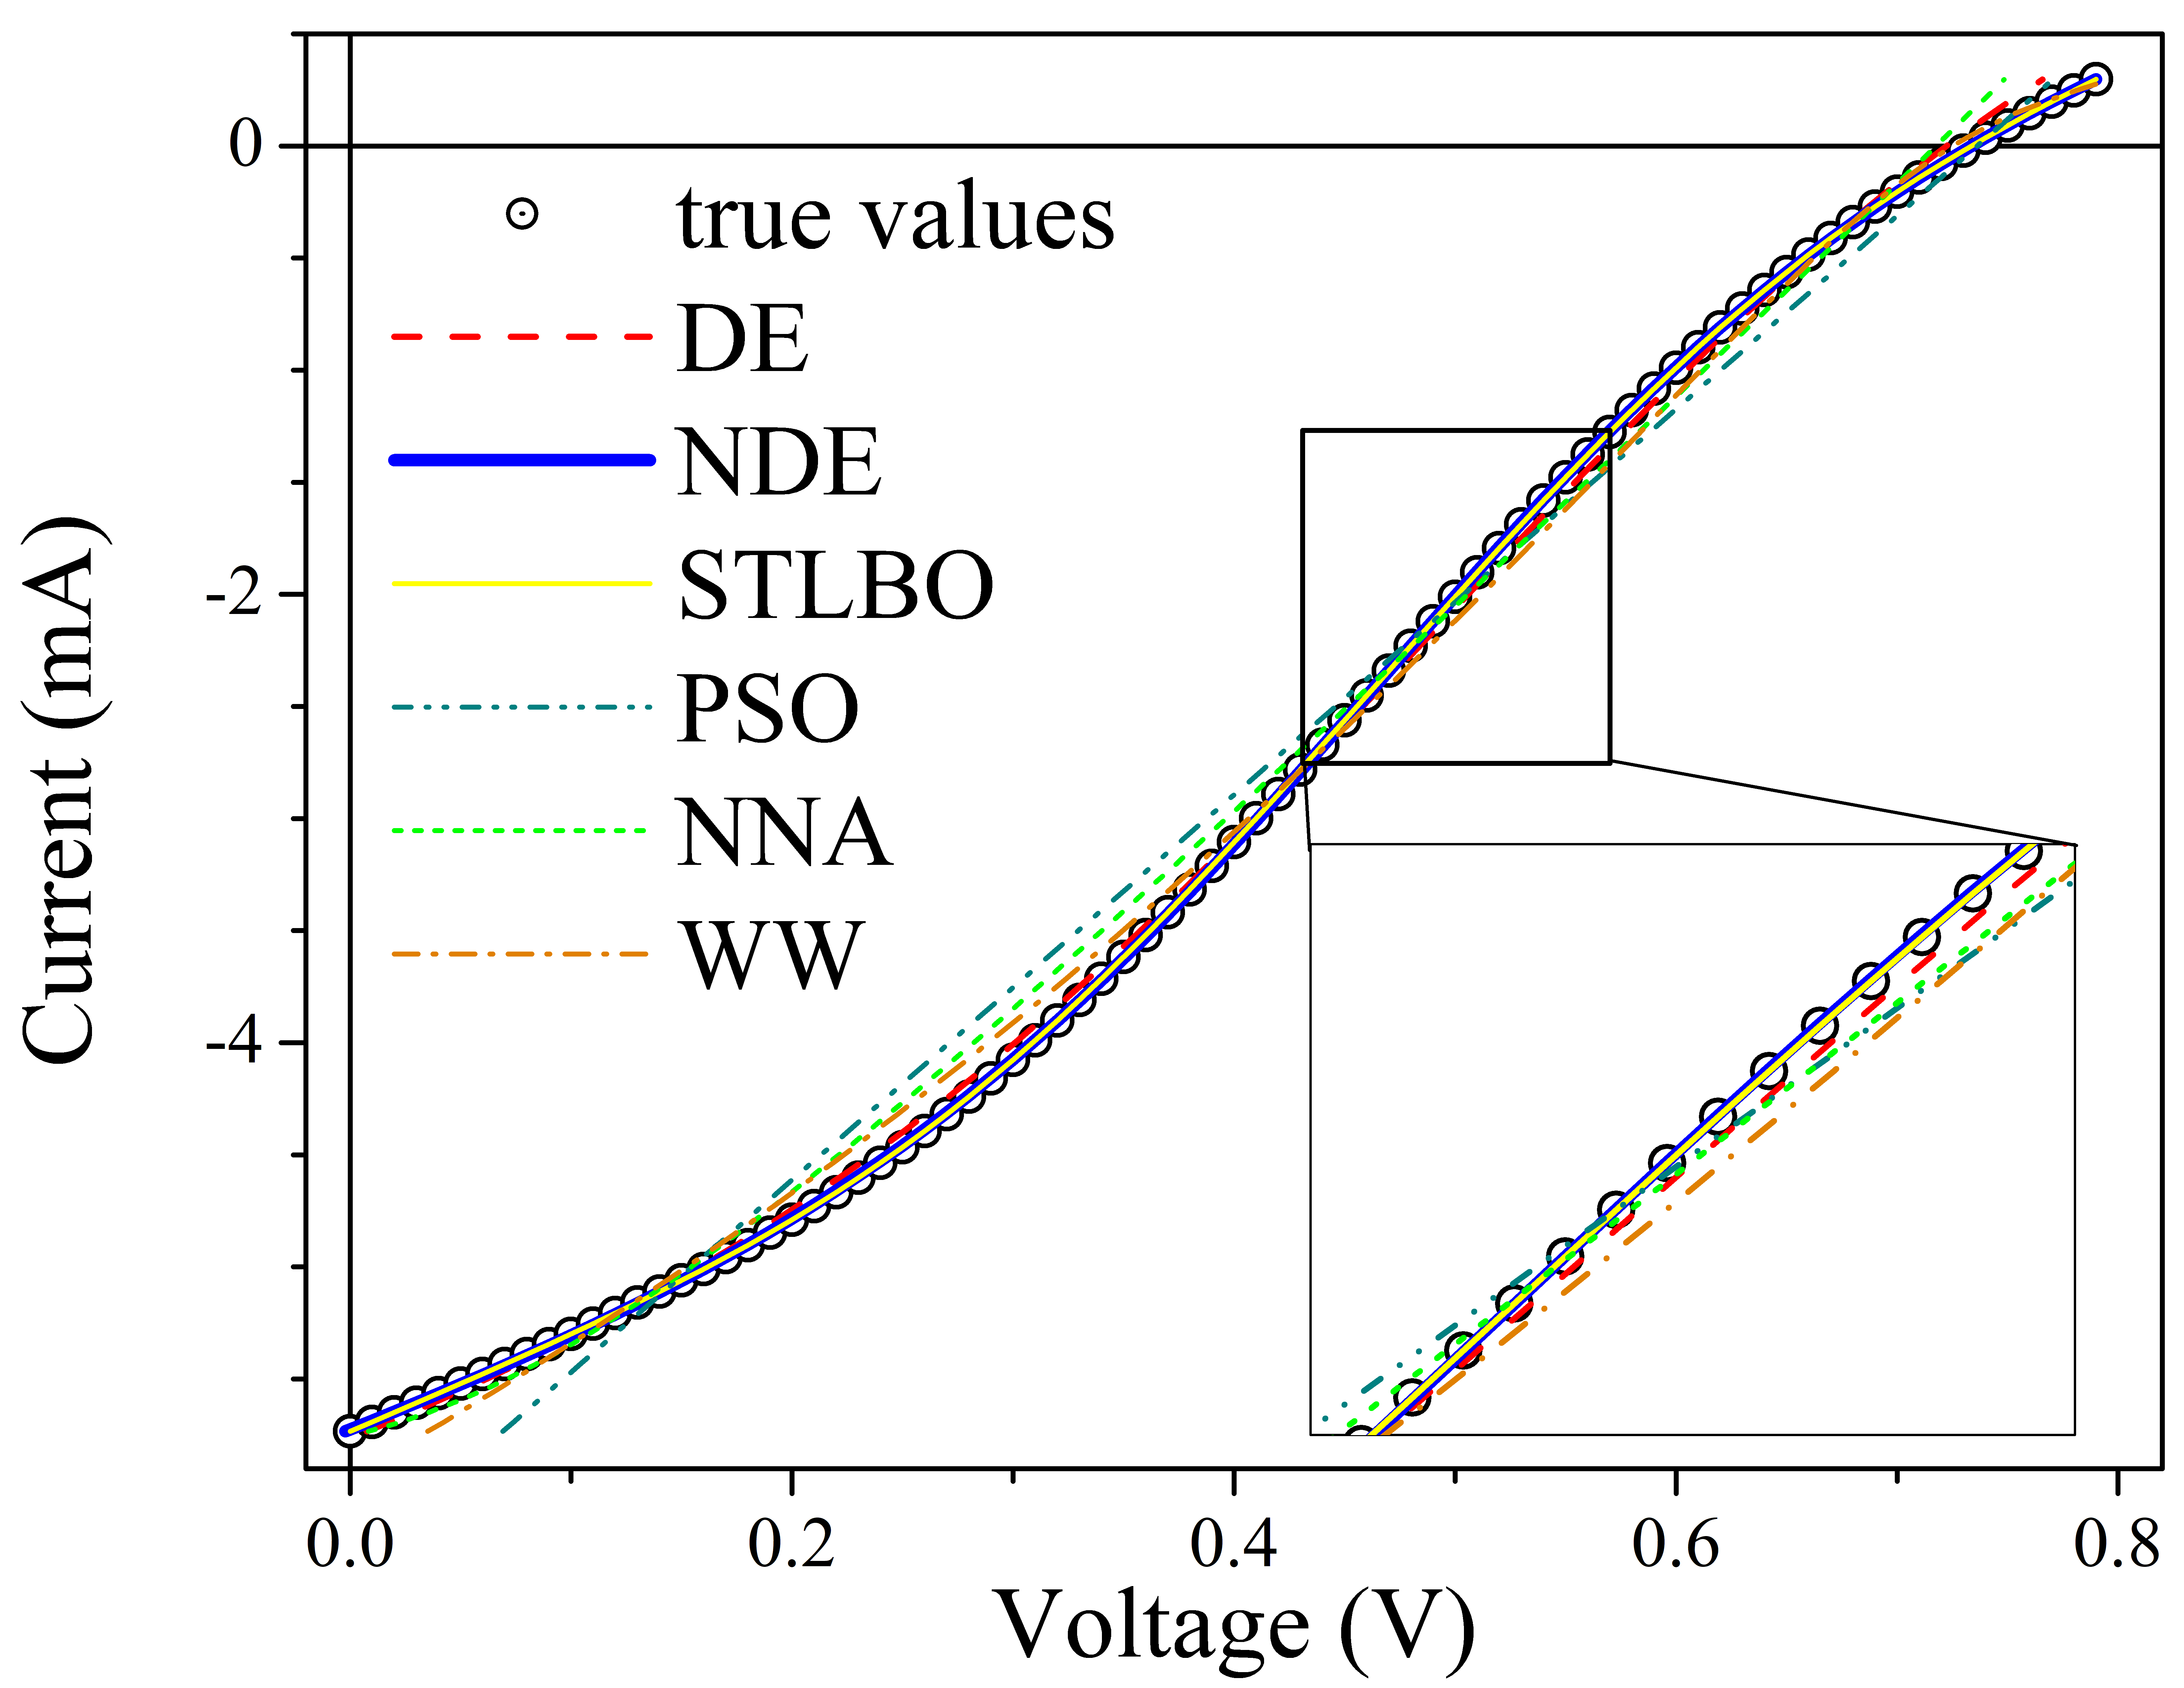
\includegraphics[width=1.0\columnwidth]{IVsimple}
	  \caption{Fitting results (lines) for the simulated current-voltage characteristic (symbols). The values from  Sec.~\ref{SingleIV} were assumed under simulation.}\label{figSigleIV}
\end{figure}

%It has been shown previously whether the ideality factor of D2 ($n_2$) is the same as that of D1
%($n_1=n_2=1.92$) or very larger than $n_1$ ($n_1=1.00$, $n_2=3.00$),
%the nonlinear least--squares method finds a set of equivalent circuit parameters that reproduces the experimental
%data of an organic photovoltaic cell.


\subsubsection{IV--set case}

%перекласти на англійську ""

%Estimation of parameters for solar cells with S--shaped current--voltage characteristics using meta--heuristic algorithms

\subsection{Meta-heuristic algorithms}\label{MHA}
In the literature, meta-heuristics are frequently categorized based on their sources of inspiration.
This categorization involves incorporating elements of true simulations and principles that incorporate stochasticity,
with the objective of emulating diverse characteristics observed in biological behavior, the lives of creatures in nature, human behavior, or natural phenomena.
On this basis, any meta-heuristic algorithm can fall into one of the following main classes \cite{WhiteShark,Gannet,Dandelion}:
evolution-based methods (emulate the principles of evolutionary behavior observed in creatures in nature by relying on the concept of survival of the fittest),
swarm intelligence--based methods (simulate the collective, dynamic, intelligent, and concerted gregarious conduct of collections of flocks or communities found in nature),
bio--based methods (use biological processes unrelated to group behavior),
chemical \& physical--based methods (originate from the physical phenomena or chemical laws that exist in the universe),
human-society--based methods (inspired by human beings, including various activities such as thinking and social behavior),
and math--based methods (borrow the mathematical functions).
Generally, there are hundreds of meta-heuristic optimization methods available.
While we acknowledge that our selection may not be fully comprehensive,
we utilized 14 methods, representing all classes mentioned above,
to tackle the parameter estimation task within the framework of the opposed two-diode model for a solar cell.
Hereafter, we provide a succinct description of each method alongside the parameters employed during the fitting process.

\emph{Differential evolution} (\textbf{DE}).
DE is one of the classical methods,
and  it is based on the natural selection law and uses the randomly generated initial population,
differential mutation, and probability crossover \cite{DEWang}.
During the implementation, we employed a penalty function suggested by Ishaque \emph{et al} \cite{P-DE_Ishaque}.
Besides, according to Wang and Ye \cite{DEWang}, the values of mutation scaling factor $F=0.8$,
crossover rate $C\!r=0.3$, and population size $N\!p=8\times D=64$ were used in this work.

\emph{Adaptive differential evolution with the Lagrange interpolation argument} (\textbf{ADELI}).
The method is based on DE, which integrates an adaptive local search scheme with Lagrange interpolation \cite{ADELI}.
This incorporation aims to enhance the exploitation capability and accelerate the convergence speed.
In ADELI, the scaling factor and crossover rate are set to self--adapting to optimize the results.
We used parameter values recommended by Huang \emph{et al} \cite{ADELI} during the implementation process.
Additionally, we set $N\!p$ to 64 for our numerical experiments.

\emph{Differential evolution with neighborhood--based adaptive evolution mechanism} (\textbf{NDE}).
The method uses a mutation strategy, which takes into account neighborhood and individual information, and an adaptive evolution mechanism \cite{NDE}.
The determination of $F$ and $C\!r$ values is achieved through the utilization of the weighted adaptive procedure \cite{Tanabe2014},
and an adaptive adjustment of the population size is implemented using a simple reduction method (from $10\times D=80$ to 5).

\emph{Success history based DE with hybridization mutation strategies and population size reduction} (\textbf{EBLSHADE}).
The method is the hybridization framework between \emph{pbest} and \emph{ord\_pbest} mutation strategies
and stores a set of $Cr$ and $F$ values that have performed well in the recent past \cite{EBLSHADE}.
A linear $N\!p$ reduction (from $18\times D=144$ to 4) is used as well.

\emph{Particle swarm optimization} (\textbf{PSO}).
It is another classic method based on observations of the social behavior of animals,
such as bird flocking, fish schooling, and swarm theory.
According to Ye et al. \cite{PSO},  the values of learning factors $l_1=l_2=2$,
the final weight and the initial weight $w_{max}=0.9$, $w_{min}=0.4$, and
$N\!p=15\times D=120$ are used in this work.

The \emph{modified artificial bee colony} (\textbf{MABC}) algorithm is based
on the intelligent foraging behavior of honey bee swarms \cite{MABC}.
The control parameters include the population size ($N\!p=8\times D=64$)
and the maximum number of generations after which each non-improved food source is to be discarded ($L_{imit}=36$).

\emph{Chaotic Whale Optimization Algorithm} (\textbf{CWOA}).
WOA draws inspiration from the hunting behavior of humpback whales \cite{WOA}.
On the other hand, CWOA employs chaotic maps to compute and dynamically adjust its internal parameters \cite{CWOA}.
In our study, we utilized the Singer chaotic map and set $N\!p=100$ for the identification of the parameters of the solar cell.

The \emph{Neural Network Algorithm} (\textbf{NNA}) is a meta-heuristic algorithm that draws inspiration from
both biological nervous systems and artificial neural networks \cite{NNA}.
The recommended \cite{NNA} value $N\!p=50$ is used in our paper.

The \emph{teaching learning based optimization} (\textbf{TLBO}) algorithm employs the concept of passing on knowledge
within a classroom.
Similar to learners acquiring knowledge from a teacher and interacting with their peers,
TLBO incorporates such interactions \cite{TLBO_Patel}.
In this study, a value of $N\!p=100$ is utilized.

\emph{Generalized oppositional teaching learning based optimization} (\textbf{GOTLBO}).
This method integrates a concept that incorporates both the current estimate
and its opposite estimate simultaneously into the original TLBO algorithm
through the initialization step and generation jumping \cite{GOTLBO}.
The values of jumping rate $J\!r=1.0$ and $N\!p=20$ were used.

\emph{Simplified teaching-learning based optimization algorithm} (\textbf{STLBO}).
In STLBO, an elite strategy is employed to improve the searching capability,
and a the chaotic map is used to enrich the uniformity of random values in the mutation phase \cite{STLBO}.
The logistic chaotic map and $N\!p=20$ were used.


\emph{Water wave optimization} (\textbf{WWO}) takes inspiration from shallow water wave models
and borrows ideas from wave propagation, refraction, and breaking \cite{WW}.
WWO is easy to implement with a small-size population, and there are four control parameters:
the maximum wave height $h_{max}$,
the wavelength reduction coefficient $\alpha$,
the breaking coefficient $\beta$,
and the maximum number $k_{max}$ of breaking directions.
According to Zheng \cite{WW}, we used
the values $h_{max}=6$, $\alpha=1.026$,  $N\!p=10$,
$k_{max}=\min(12,D/2)=4$, and $\beta$ linearly decreased from 0.25 to 0.001.

\emph{Improved JAYA} (\textbf{IJAYA}).
Jaya algorithm is based on the concept
that the solution obtained for a given problem should move toward the best solution and should
avoid the worst solution and does not require any algorithm-specific parameter \cite{JAYA}.
In IJAYA, a self-adaptive weight is introduced to adjust the tendency of approaching the best solution
and avoiding the worst solution;
an experience-based learning strategy is employed to maintain the population diversity and enhance the exploration ability,
and a chaotic elite learning method is proposed to refine the quality of the best solution in each generation \cite{IJAYA}.
The logistic chaotic map and $N\!p=4\times D=32$ were used.

\emph{Improved sine cosine algorithm} (\textbf{ISCA}).
SCA based on simulating the behaviors of sine and cosine mathematical functions \cite{SCA}.
ISCA implementation included a modified position-updating equation based on inertia weight
($w_{start}=1$, $w_{end}=1$),
a nonlinear conversion parameter strategy based on the Gaussian function
($a_{start}=2$, $a_{end}=0$) \cite{ISCA2},
the creation of the opposite population to jump out from the local optima with $J\!r=0.1$ \cite{ISCA3},
a greedy selection, and $N\!p=30$.

The majority of the utilized algorithms demonstrate excellent performance when
it comes to parameter estimation of solar cells within conventional models (single or double diode) \cite{CWOA,DEWang,GOTLBO,IJAYA,MABC,PSO,STLBO,TLBO_Patel,LSHADE,IWOA}.

The performance of the extracted parameters is evaluated using the fitness function at
every iteration.
In our investigation, two fitness function were used:
\begin{equation}
\label{eqFae}
F_\mathrm{AE}(Y)= \sum_{k=1}^p \left|V^\mathrm{tr}(I_k)-V^\mathrm{cal}(I_k,Y)\right|\,,
\end{equation}
\begin{equation}
\label{eqFse}
F_\mathrm{SE}(Y)= \sum_{k=1}^p \left[V^\mathrm{tr}(I_k)-V^\mathrm{cal}(I_k,Y)\right]^2\,,
\end{equation}
where
$V^\mathrm{tr}(I_k)$ is the simulated value of voltage at current $I_k$,
$V^\mathrm{cal}(I_k,Y)$ is the calculated values of voltage, which can be obtained
by Eqs.~(\ref{eqIV_g})--(\ref{eqx2}),
for given set of parameters (i.e. $Y = \{I_{01},n_1,R_\mathrm{p1},I_{02},n_2,R_\mathrm{p2},R_\mathrm{s},I_\mathrm{ph}\}$)
at current $I_k$,
and $p$ is the total number of voltage steps in the IV characteristic.


%The numbers of independent algorithmic runs are
%equal to 30 utilized to generate the statistical results.

Each algorithm was run 51 times with different random seed for each simulated IV curves.
The search ranges were set as follows:

\noindent
$I_{01}(\mathrm{mA})\in[10^{-13},1]$,
$n_1\in[0.5,50]$,
$R_\mathrm{p1}(\Omega)\in[10,10^6]$,
$I_{02}(\mathrm{mA})\in[10^{-7},10]$,
$n_2\in[0.5,50]$,
$R_\mathrm{p2}(\Omega)\in[10,5\cdot10^4]$,
$R_\mathrm{s}(\Omega)\in[0.1,1000]$,
$I_\mathrm{ph}(\mathrm{mA})\in[10^{-3},100]$.
%\begin{eqnarray}
%\label{eqSR}
%I_{01}(\mathrm{mA})&\in&[10^{-13},1]\nonumber, \\
%n_1&\in&[0.5,50]\nonumber, \\
%R_\mathrm{p1}(\Omega)&\in&[10,10^6]\nonumber, \\
%I_{02}(\mathrm{mA})&\in&[10^{-7},10]\nonumber, \\
%n_2&\in&[0.5,50]\nonumber, \\
%R_\mathrm{p2}(\Omega)&\in&[10,5\cdot10^4]\nonumber, \\
%R_\mathrm{s}(\Omega)&\in&[0.1,1000]\nonumber, \\
%I_\mathrm{ph}(\mathrm{mA})&\in&[10^{-3},100]\nonumber .
%\end{eqnarray}

\subsection{Evaluation criteria}\label{EvalCr}


%To appropriately evaluate the performance of the
%proposed NNA compared with the other state-of-art algorithms,
%four quality indicators are utilized. The first one is the value-based
%method which is the solution quality in terms of four performance
%metrics including the best, average, median, worst, and standard
%deviation (SD).
%The second metric is the rank-based method, which have been
%suggested by different authors in the literature. In this paper, the
%Friedman test [37] which is a nonparametric statistical test is
%used to distinguish the differences among reported algorithms.
%Therefore, the average rankings of the algorithms according to the
%Friedman test are reported.
%The third and fourth metrics are Kruskal-Wallis test [38] and
%Multiple Comparison Test [39]. Tables 8–13 tabulate the obtained
%optimization results using different optimizers for the benchmarks
%given in Tables 5 and 6 with dimensions of 50–200. Looking at
%Tables 8–13, performance of well-used optimizers such as GA, PSO,
%HS has not surpassed the results of recent optimizers for the most
%reported functions. Therefore, the competition is mostly among
%recent developed optimization methods

%With the aim of obtaining rigorous and fair conclusion, two other
%statistical tests have been carried out in this research including the
%Kruskal-Wallis H test [38] and Multiple Comparison Test [39]. These
%tests have been conducted for proving if there are significant differences in the results obtained by all methods and each method
%compared with the another.


%For each benchmark function, individual optimizer runs Nruns
%times starting from different populations randomly generated and
%the following seven evaluation indicators are computed per optimizer:
%1. Mean fitness: is an average value of all the solutions in
%the final sets obtained by an optimizer in some individual
%runs [35].
%2. Statistical standard deviation (std): is used to ensure that the
%optimizer convergences to the same optimal and ensures
%repeatability of the results. It is computed over all the sets
%of final solutions obtained by an optimizer in a number of
%individual runs [36].
%3. Wilcoxon rank sum test: assigns a rank to all the scores
%considered as one group and then sums the ranks of each
%group [37]. The rank-sum test is often described as the
%nonparametric version of the t test for two independent
%groups.
%4. T-test: is statistical significance shows despite whether the
%contrast between the two groups’ midpoints in all possibility
%mirrors a real distinction in the population from the groups
%were inspected [38].
%5. Run time average: is the average run time in seconds for an
%individual optimizer on a given function. The results were
%conducted on 64-bit windows 10 computer with i7 core
%3.6 GHz and 8 GB RAM.

Table 17
Run time average for the different optimizers adopted in the study for the different functions


\section{Simulation results and analysis}\label{Result}


%In metaheuristic algorithms, a different termination can be
%defined. For instance, a termination condition can be a specific
%number of iterations, constraints on the number of function evaluations, a specific rate of precision, a specific time, no sign of
%change in solutions after a specific number of iterations, or a combination of these cases. In the proposed method, the termination
%condition was defined as imposing constraints on the number
%of function evaluations (MaxFEs) and reaching a specific rate of
%precision.

%3.5. Computational time analysis
%Another evaluation criterion used to compare the algorithms’
%performance is to compare their execution time in terms of
%solving different problems. The mean sum of 30 different runs
%in each algorithm is shown in Fig. 10 to solve 39 functions
%(unimodal, multimodal, fixed dimension multimodal, composite
%functions and CEC2019 functions). According to the figure, execution time of ICO is less than execution time of known and
%efficient algorithms like DE, LASHADE-SPACMA, LSHADE-cnEpSin
%and HGSO.


%

%The
%experiments were implemented in Matlab and run on Windows
%7 operative system with 64-bit support with a 2.0 GHz Intel
%dual-core processor and 4 GB RAM.

%the maximum number of function evaluations (FEs) is set to 3000  D.
%The
%quality of them is evaluated in terms of the objective function
%(Root Mean Square Error)
%
%CPU time

%For all the algorithms, a population size and maximum iteration
%equal to 30 and 500 have been utilized. The number of search
%agents n and number of iteration T are commonly set based on trial
%and error basis and should be proportional to the size of the search
%space and the complexity of the fitness function. In this work, we
%adopted the same setting for n and T as in the original paper by
%in Mirjalili

%перекласти на англійську "Переважна більшість використаних алгоритмів показують гарні результати при оцінці параметрів сонячних елементів в межах звичних моделей "

%покращити стилістику, виправити граматичні та стилістичні помилки, використовуючи стиль наукової статті "The method is based on DE by incorporating an adaptive local search scheme with Lagrange interpolation to enhance the exploitation capability to accelerate the convergence speed."


%3.2.6. Wilcoxon signed-rank test
%In order to show the obtained results of ICO that is significantly different from the other randomized algorithms, the
%Wilcoxon Signed-Rank Test was used for pairwise comparison.
%The test was performed by using the global minimum values
%obtained by performing 30 runs for problem based pairwise comparison of the algorithms. The significance value α was chosen to
%be 0.05 with null hypothesis H0; that is, there is no difference
%between the median of the solutions obtained after the same
%test problem is executed by algorithms A and B, i.e. median (A)
%= median(B). Also, to determine whether algorithm A yielded
%statistically the better solution than algorithm B or whether alternative hypothesis was valid, the sizes of the ranks provided
%by the Wilcoxon Signed-Rank test (T+ and T−) were thoroughly
%examined.
%The non-parametric statistical results of the ICO algorithm
%versus other algorithms based on the Wilcoxon Signed-Rank Test
%with the statistical significance level α = 0.05 are also summarized in Tables 13–17. In these tables, ‘+’ indicated that the null
%hypothesis H0 was rejected and ICO performed better, while ‘−’
%indicated that the null hypothesis H0 was rejected; however, ICO
%performed worse. The ‘=’ indicates a failure to reject the null
%hypothesis, and also there is no statistical difference between the
%two algorithms. The counts of statistical significant cases (+/−/=)
%are presented in the last row of Tables 13–17
%The Wilcoxon Signed-Rank Test results for each test category
%are presented in Table 18. In this table, each cell shows total count
%of three statistical significance cases (+/ = /−) in the pairwise
%comparison. The results show that ICO can achieve statistically
%better results than comparison algorithms except SASS, with a
%level of significance α = 0.05. However, the numerical results
%provided for some algorithms such as DE in fixed-dimension
%multimodal functions is not sufficient to make a statistically
%convincing inference. With regard to Wilcoxon Signed-Rank Test
%in Table 18, the performance success of ICO in fixed-dimension
%multimodal functions is relatively low compared to others. This
%fits ‘‘No-Free-Lunch’’ (NFL) theorem.


%див
%Table 13
%The results of two-sided Wilcoxon Signed-Rank test with α = 0.05 for (F1–F7), with 30 dimensions.
%ApplSoftComp_115_108126
%Table 19
%Ranking of algorithm according to Friedman ranking based on mean error value. (FR: Friedman Ranking)

%3.2.7. Friedman ranking (FR) test
%The Friedman test was employed to compare the proposed
%method with other state-of-art algorithms presented in this paper. It is a nonparametric test and equivalent to the analysis
%of variance with repetitive sizes (within groups). This test is
%utilized to compare mean of ranks between k variables (groups).
%According to the ranking performed through the Friedman test,
%the proposed method was ranked as the highest in all existing
%methods by considering 39 different test functions. Table 19
%shows the rank of each method. The following equation can be
%employed to determine the superiority of ICO in other methods:
%(new_value − original_value)/|original_value| × 100 (24)
%Where new_value shows the rank of ICO when original_value
%indicates the rank of each technique used to calculate the superiority of ICO to that method. According to the results, ICO could
%outperform EO, GWO, WOA, MFO, PSO, DE, GSA, SSA, SHO, GAMPC, LSHADE, LSHADE-cnEpSin, LSHADE-SPACMA, SASS, AOA and
%HGSO 28%, 47%, 53%, 61%, 47%, 21%, 44%, 52%, 56%, 47%, 31%, 27%,
%22%, 7%, 61% and 52% respectively in 39 benchmark functions. The
%P-value of Friedman rank test was reported 7.2868e−25. Since
%it is smaller than 0.05, it can be concluded that the results of
%different algorithms are significantly different.


%Table 15
%Sum of average ranking using Friedman test for applied optimization methods.
%Methods Total Average Ranking by Friedman Test (Rank)

%As can be seen from Table 15, the NNA has been placed at first
%rank and the DE and TLBO have been located at the second and third
%ranks, respectively. The RS, as expected, is the worst algorithm for
%solving the reported benchmarks and could not even find acceptable results for all cases (see Table 14). Looking at huge gaps in the
%obtained optimization results by the NNA and RS, we can conclude
%that the NNA is not based on the simple random search even in its
%exploration phase.


%ApplSoftComp_71_p747
%The second column of Table 16 represent the methods which
%are compared. The third and fifth columns show lower and upper
%limits (LL and UL) for 95% confidence intervals for the true mean
%difference. The fourth column show the difference between the
%estimated method means. The sixth column (i.e., last column) contains the p-value for a hypothesis test that the corresponding mean
%difference is equal to zero obtained by Kruskal-Wallis H test with
%˛ = 0.05. Figs. 6–9 depict the boxplot and multiple comparison plot
%among the considered optimizers for all considered benchmarks.
%In Figs. 6–9, vertical axis in Kruskal-Wallis H test is the value of
%objective function obtained by the studied optimizers

%The obtained
%p-values in last column of Table 16 prove this comparison. For
%instance, looking at F17 in Fig. 9, we can see the NNA statistically
%has outperformed six optimizers (i.e., TLBO, WCA, ICA, PSO, DE, and
%CMA-ES), while the optimization results obtained by the CS, GSA,
%HS, GA, and SA are the same with no significance difference. Lines
%right side of the NNA (i.e., blue lines) show the methods which are
%not significantly better than the NNA, while lines left side of the
%NNA show the methods which are statistically better than the NNA
%for a specific benchmark.
%Furthermore, Table 17 tabulates the obtained optimization
%results along with their statistical tests and ranking for dimension
%200 (˛ = 0.05) for 1E + 06 NFEs. Due to the limitation of execution
%time, only the TLBO and GSA have been selected in the comparison
%pool.
%From Table 17, the NNA obtained the lower total average ranking
%which shows its overall efficiency compared with the considered
%optimizers. For the most cases, the NNA has been placed in the first
%or second ranks. Now, it is interesting to see the performance of
%the NNA over few iterations. Therefore, Figs. 10 and 11 display the
%total cost reduction history of reported optimizers over only 200
%iterations between selected optimizer given in Table 17. It is worth
%mentioning that all reported optimizers start with a random initial
%population between the lower and upper bounds.


%Table 18,19




% Numbered list
% Use the style of numbering in square brackets.
% If nothing is used, default style will be taken.
%\begin{enumerate}[a)]
%\item
%\item
%\item
%\end{enumerate}

% Unnumbered list
%\begin{itemize}
%\item ff
%\item ff
%\item ff
%\end{itemize}

% Description list
%\begin{description}
%\item[]
%\item[]
%\item[]
%\end{description}

% Figure
%\begin{figure}[<options>]
%	\centering
%		\includegraphics[<options>]{}
%	  \caption{}\label{fig1}
%\end{figure}


\begin{table}[<options>]
\caption{}\label{tbl1}
\begin{tabular*}{\tblwidth}{@{}LL@{}}
\toprule
  &  \\ % Table header row
\midrule
 & \\
 & \\
 & \\
 & \\
\bottomrule
\end{tabular*}
\end{table}

% Uncomment and use as the case may be
%\begin{theorem}
%\end{theorem}

% Uncomment and use as the case may be
%\begin{lemma}
%\end{lemma}

%% The Appendices part is started with the command \appendix;
%% appendix sections are then done as normal sections
%% \appendix

%\section{}\label{}





% To print the credit authorship contribution details
%\printcredits

%% Loading bibliography style file
%\bibliographystyle{elsarticle-num-names}
\bibliographystyle{model1-num-names}
\bibliography{olikh_Methods}


\end{document}

